\documentclass[12pt,a4paper]{article}

\usepackage[utf8]{inputenc}
\usepackage[T5]{fontenc}
\usepackage{amsmath, amssymb}
\usepackage{bm}
\usepackage{graphicx}
\usepackage{booktabs}
\usepackage{geometry}
\usepackage{hyperref}
\usepackage{enumitem}
\usepackage{float}
\usepackage{multirow}

\geometry{right=2cm, left=3cm, top=2cm, bottom=2.5cm}
\renewcommand{\baselinestretch}{1.2}
\graphicspath{{../../thesis/figures/}{../sm2/figures/}}

\newcommand{\R}{\mathbb{R}}
\newcommand{\T}{\mathsf{T}}
\DeclareMathOperator{\diag}{diag}

\begin{document}

% ================================================================
% HEADER
% ================================================================
\begin{center}
    {\Large\bfseries BÁO CÁO TIẾN ĐỘ LUẬN VĂN THẠC SĨ} \\[10pt]
    {\large\bfseries Đề tài: Điều khiển tối ưu thích nghi dựa trên Quy hoạch động\\
    hội tụ cố định thời gian cho Robot di động hai bánh} \\[14pt]
    \begin{tabular}{rl}
        \textbf{Học viên:}      & Nguyễn Thành Trung \\
        \textbf{GVHD:}          & PGS.TS. Nguyễn Hoài Nam \\
        \textbf{Chuyên ngành:}  & Kỹ thuật Điều khiển và Tự động hóa \\
                                & Đại học Bách khoa Hà Nội \\
        \textbf{Ngày:}          & 26/05/2026 \\
    \end{tabular}
\end{center}

\vspace{6pt}\hrule\vspace{16pt}

% ================================================================
\section{Tóm tắt đề tài và mục tiêu nghiên cứu}
% ================================================================

\subsection{Bối cảnh}

Robot di động hai bánh vi sai (Wheeled Mobile Robot -- WMR) là nền tảng phổ biến trong các ứng dụng tự hành, logistics nhà kho, và robot dịch vụ. Bài toán bám quỹ đạo cho WMR đặt ra nhiều thách thức do tính phi tuyến, ràng buộc nonholonomic, và sự hiện diện của nhiễu loạn cùng bất định mô hình trong thực tế. Các phương pháp điều khiển truyền thống như Backstepping hay Sliding Mode Control đã được nghiên cứu rộng rãi, tuy nhiên vấn đề tối ưu hóa hiệu năng điều khiển theo nghĩa chi phí năng lượng vẫn còn hạn chế.

Gần đây, Wang và cộng sự (IEEE RA-L, 2025)~\cite{Wang2025} đã đề xuất phương pháp điều khiển tối ưu dựa trên Quy hoạch động thích nghi (Adaptive Dynamic Programming -- ADP) với tính chất hội tụ cố định thời gian (fixed-time convergence). Phương pháp này đảm bảo sai số bám và sai số ước lượng trọng số hội tụ về \textit{lân cận} của không trong thời gian cố định, không phụ thuộc điều kiện đầu (practical fixed-time). Tuy nhiên, công trình gốc chỉ xét mô hình \textbf{kinematic} đơn giản, bỏ qua hoàn toàn động lực học (dynamic) của robot.

\subsection{Mục tiêu nghiên cứu}

Luận văn này mở rộng phương pháp ADP Fixed-time từ mô hình kinematic-only sang \textbf{kiến trúc điều khiển 2 vòng} (dual-loop) bao gồm cả kinematic và dynamic cho WMR, nhằm tiến gần hơn đến ứng dụng thực tế.

\subsection{Bốn đóng góp chính}

\begin{enumerate}
    \item \textbf{Kiến trúc 2 vòng lồng nhau:} Vòng ngoài sử dụng ADP Fixed-time (hoặc các bộ điều khiển so sánh) để sinh vận tốc tham chiếu; vòng trong sử dụng Dynamic Backstepping (Fierro \& Lewis, 1997)~\cite{Fierro1997} để chuyển đổi sang mô-men điều khiển thực tế, có tính đến quán tính, ma sát và giới hạn mô-men.

    \item \textbf{Điều chỉnh tham số robust cho dual-loop:} Các hệ số robust (fractional power, cubic terms) trong Wang et al. được thiết kế cho kinematic-only. Khi kết hợp với vòng trong đã reject nhiễu, các hệ số này phải giảm mạnh để tránh phát tán -- riêng $\beta$ từ $10^5$ xuống $0{,}15$. Luận văn trình bày quy trình điều chỉnh chi tiết, phân tích nguyên nhân, và \textbf{nêu rõ cái giá phải trả} đối với đảm bảo hội tụ cố định thời gian.

    \item \textbf{So sánh toàn diện 5 phương pháp điều khiển:} Backstepping (BS), ADP Actor-Critic (AC), Sliding Mode Control (SMC), Critic-only Concurrent Learning (CL), và ADP Fixed-time (ADP-FT) được đánh giá trên 3 loại quỹ đạo với cùng điều kiện mô phỏng.

    \item \textbf{Phân tích robustness:} Khảo sát ảnh hưởng của bất định khối lượng (0--40\%) và nhiễu ngoài (0--60\% mô-men cực đại) lên hiệu năng các bộ điều khiển.
\end{enumerate}

% ================================================================
\section{Kiến trúc hệ thống}
% ================================================================

\subsection{Sơ đồ điều khiển 2 vòng}

Kiến trúc điều khiển gồm hai vòng lồng nhau:

\begin{center}
\begin{tabular}{|c|c|c|}
\hline
\textbf{Vòng ngoài (Kinematic)} & \textbf{Vòng trong (Dynamic)} & \textbf{Đối tượng (Plant)} \\
\hline
1. Backstepping (BS) & & \\
2. ADP Actor-Critic (AC) & Dynamic Backstepping & WMR mô hình đầy đủ \\
3. Sliding Mode (SMC) & (Fierro \& Lewis 1997) & 5 trạng thái \\
4. Critic-only CL & $\boldsymbol{\tau} = B^{-1}[M(\cdot)+F]$ & + nhiễu $d(t)$ \\
5. ADP Fixed-time (FT) & & \\
\hline
\end{tabular}
\end{center}

\noindent
\textbf{Vòng ngoài} nhận sai lệch quỹ đạo $(e_x, e_y, e_\theta)$ và sinh ra tín hiệu vận tốc tham chiếu $(v_c, \omega_c)$. \textbf{Vòng trong} nhận sai lệch vận tốc $(v - v_c, \omega - \omega_c)$ và tính mô-men bánh trái/phải $(\tau_L, \tau_R)$ để bám theo vận tốc yêu cầu, đồng thời bù các thành phần phi tuyến và ma sát.

Nhiễu ngoài $d(t) = A \cdot \tau_\text{max} \cdot \sin(30t)$ được cộng trực tiếp vào mô-men trên cả hai kênh, mô phỏng nhiễu loạn tần số cao trong thực tế (theo yêu cầu của thầy hướng dẫn sau Seminar 1).

\subsection{Mô hình robot di động}

Mô hình WMR gồm 5 biến trạng thái $\mathbf{q} = [x, y, \theta, v, \omega]^\T$, trong đó $(x, y)$ là tọa độ, $\theta$ là góc hướng, $v$ là vận tốc tịnh tiến, $\omega$ là vận tốc góc. Các thông số mô hình:

\begin{center}
\begin{tabular}{lll}
\toprule
\textbf{Thông số} & \textbf{Ký hiệu} & \textbf{Giá trị} \\
\midrule
Khối lượng robot & $m$ & 10\,kg \\
Mô-men quán tính & $I$ & 0.5\,kg$\cdot$m$^2$ \\
Bán kính bánh xe & $r$ & 0.05\,m \\
Nửa khoảng cách trục & $L$ & 0.15\,m \\
Mô-men cực đại mỗi bánh & $\tau_\text{max}$ & 20\,N$\cdot$m \\
\bottomrule
\end{tabular}
\end{center}

Phương trình động lực học:
\begin{align}
    \dot{x} &= v\cos\theta, \quad \dot{y} = v\sin\theta, \quad \dot{\theta} = \omega \\
    m\dot{v} &= \frac{1}{r}(\tau_R + \tau_L) + d_v(t) \\
    I\dot{\omega} &= \frac{L}{r}(\tau_R - \tau_L) + d_\omega(t)
\end{align}
trong đó $d_v(t), d_\omega(t)$ là nhiễu ngoài tác động lên kênh tịnh tiến và kênh quay.

% ================================================================
\section{Kết quả Seminar 1: Actor-Critic ADP trên mô hình Kinematic}
% ================================================================

Seminar 1 (tháng 3/2026) tập trung triển khai và so sánh phương pháp ADP Actor-Critic (Vamvoudakis \& Lewis, 2010)~\cite{Vamvoudakis2010} với Backstepping trên \textbf{mô hình kinematic đơn giản} (chưa có vòng trong dynamic). Mạng Actor và Critic sử dụng cấu trúc 2 lớp với hàm kích hoạt polynomial.

Kịch bản mô phỏng: hai quỹ đạo tham chiếu (đường tròn bán kính 1\,m và đường thẳng), thời gian $T = 120$\,s, không có nhiễu ngoài. Ba phương pháp được so sánh: BS (Backstepping), AC+PE (Actor-Critic có tín hiệu Persistence of Excitation), và AC (không PE).

\begin{table}[H]
\centering
\caption{Kết quả Seminar 1: Mô hình kinematic ($T=120$\,s, không nhiễu)}
\begin{tabular}{llrr}
\toprule
\textbf{Quỹ đạo} & \textbf{Phương pháp} & $J_c$ & $z_\text{rms}$ (10\,s cuối) \\
\midrule
Đường tròn & BS          & 7.39  & $\approx 0$ \\
Đường tròn & AC + PE     & 17.06 & 0.0004 \\
Đường tròn & AC (không PE)  & 27.96 & 0.0019 \\
\midrule
Đường thẳng & BS          & 7.06  & $\approx 0$ \\
Đường thẳng & AC + PE     & 152.5 & 0.4516 \\
Đường thẳng & AC (không PE)  & 114.7 & 0.3608 \\
\bottomrule
\end{tabular}
\end{table}

\textbf{Phân tích kết quả:}
\begin{itemize}
    \item \textbf{Đường tròn:} AC+PE hoạt động ổn định ($J_c = 17.06$), gấp 2.3 lần BS nhưng sai số xác lập rất nhỏ. AC không PE kém hơn ($J_c = 27.96$) do trọng số Critic chưa hội tụ đầy đủ.

    \item \textbf{Đường thẳng:} Cả hai phiên bản AC đều hoạt động kém ($J_c > 100$). Nguyên nhân: trên đường thẳng, vận tốc góc tham chiếu $\omega_r = 0$, dẫn đến tín hiệu PE không đủ phong phú để kích thích hệ thống. Đặc biệt, \textbf{PE phản tác dụng} trên đường thẳng: AC+PE ($J_c = 152.5$) kém hơn AC không PE ($J_c = 114.7$) do tín hiệu PE gây nhiễu loạn không cần thiết.

    \item \textbf{Kết luận SM1:} Phương pháp Actor-Critic cần warm start (khởi tạo trọng số ban đầu tốt) và phụ thuộc nặng vào PE. Hạn chế này thúc đẩy nghiên cứu phương pháp Critic-only trong SM2.
\end{itemize}

% ================================================================
\section{Kết quả Seminar 2: Critic-only với Concurrent Learning}
% ================================================================

Seminar 2 (tháng 4/2026) triển khai phương pháp Critic-only kết hợp Concurrent Learning (CL) theo Chowdhary \& Johnson (2010)~\cite{Chowdhary2010}. Ý tưởng chính: loại bỏ hoàn toàn mạng Actor, chỉ sử dụng mạng Critic duy nhất. Thay vì dựa vào tín hiệu PE để đảm bảo hội tụ, CL lưu trữ dữ liệu quá khứ (experience replay) và sử dụng đồng thời dữ liệu hiện tại + lịch sử để cập nhật trọng số. Điều này loại bỏ điều kiện PE --- vốn là hạn chế lớn nhất của Actor-Critic.

\begin{table}[H]
\centering
\caption{Kết quả Seminar 2: CL thay thế PE (kinematic, $T=120$\,s, không nhiễu)}
\begin{tabular}{llrr}
\toprule
\textbf{Quỹ đạo} & \textbf{Phương pháp} & $J_c$ & $z_\text{rms}$ (10\,s cuối) \\
\midrule
Đường tròn & BS          & 1.35  & $\approx 0$ \\
Đường tròn & AC + PE     & 7.64  & 0.0003 \\
Đường tròn & CL (không PE)  & 8.31  & 0.0005 \\
\midrule
Đường thẳng & BS          & 1.29  & $\approx 0$ \\
Đường thẳng & AC + PE     & 72.71 & 0.3000 \\
Đường thẳng & CL (không PE)  & \textbf{5.60}  & 0.0042 \\
\bottomrule
\end{tabular}
\end{table}

\textbf{Phân tích kết quả:}
\begin{itemize}
    \item \textbf{Đường tròn:} CL đạt $J_c = 8.31$, chỉ chênh 8.8\% so với AC+PE ($J_c = 7.64$). Cả hai phương pháp ADP đều còn khoảng cách so với BS ($J_c = 1.35$), do quá trình học trực tuyến tiêu tốn năng lượng trong giai đoạn đầu.

    \item \textbf{Đường thẳng:} CL \textbf{vượt trội hoàn toàn} với $J_c = 5.60$, gấp 13 lần tốt hơn AC+PE ($J_c = 72.71$). CL hoạt động ổn định nhờ cơ chế experience replay cung cấp đủ thông tin ngay cả khi quỹ đạo tham chiếu nghèo nàn ($\omega_r = 0$).

    \item \textbf{Kết luận SM2:} Concurrent Learning là giải pháp hiệu quả thay thế PE. CL chỉ cần 1 mạng nơ-ron (Critic), không cần tín hiệu kích thích bổ sung, và hoạt động ổn định trên mọi loại quỹ đạo.
\end{itemize}

\begin{figure}[H]
    \centering
    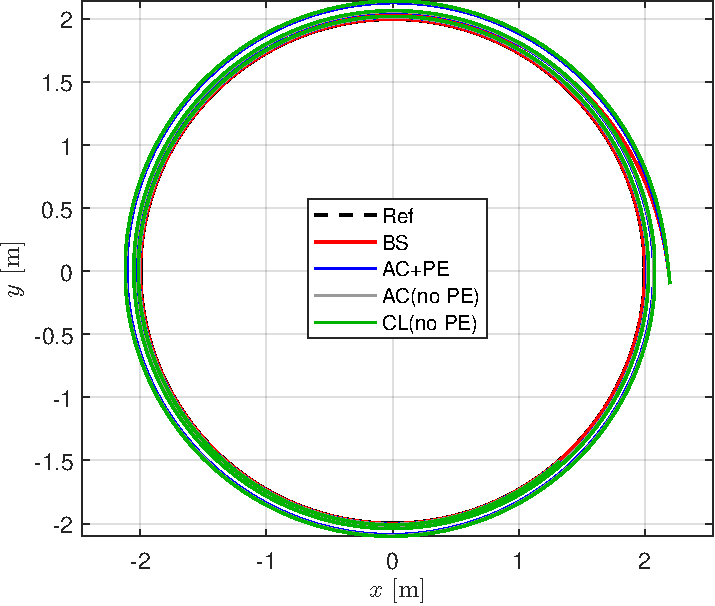
\includegraphics[width=0.75\textwidth]{sm2_xy_circle.pdf}
    \caption{SM2: Quỹ đạo bám đường tròn --- so sánh BS, AC+PE, CL (kinematic).}
    \label{fig:sm2_xy_circle}
\end{figure}

% ================================================================
\section{Kết quả chính: Mô hình đầy đủ, 5 phương pháp điều khiển}
% ================================================================

Đây là phần kết quả chính của luận văn, thực hiện trên \textbf{mô hình đầy đủ 5 trạng thái} với kiến trúc 2 vòng. Tất cả 5 phương pháp vòng ngoài đều sử dụng chung bộ điều khiển vòng trong Dynamic Backstepping.

\subsection{Phần A: So sánh 3 quỹ đạo $\times$ 5 phương pháp ($T=60$\,s, nhiễu 20\%)}

Điều kiện mô phỏng: thời gian $T = 60$\,s, nhiễu ngoài $d(t) = 0.2 \cdot \tau_\text{max} \cdot \sin(30t)$ trên cả hai kênh mô-men. Ba quỹ đạo tham chiếu: đường tròn (bán kính 1\,m, $\omega_r = 0.5$\,rad/s), đường thẳng ($v_r = 0.5$\,m/s, $\omega_r = 0$), và hình số 8 (lissajous).

Chỉ số đánh giá:
\begin{itemize}[nosep]
    \item $J_c$: Tổng chi phí tích lũy (cumulative cost), bao gồm sai lệch bám + năng lượng điều khiển.
    \item $J_e$: Chi phí sai lệch thuần túy (chỉ tính tracking error).
    \item $z_\text{rms}$: Sai số RMS trung bình trong 5 giây cuối cùng, đánh giá chất lượng xác lập.
\end{itemize}

\begin{table}[H]
\centering
\caption{So sánh toàn diện 5 phương pháp (mô hình đầy đủ, dual-loop, $T=60$\,s, nhiễu 20\%)}
\begin{tabular}{llrrr}
\toprule
\textbf{Quỹ đạo} & \textbf{Phương pháp} & $J_c$ & $J_e$ & $z_\text{rms}$ (5\,s cuối) \\
\midrule
\multirow{5}{*}{Đường tròn}
    & BS                        &  90.1 &  6.62 & 0.000 \\
    & ADP-AC                    & 121.2 & 11.01 & 0.113 \\
    & SMC                       & 555.5 & 29.23 & 0.743 \\
    & CL                        & 101.1 &  9.11 & 0.058 \\
    & \textbf{ADP-FT}           & \textbf{85.2} & \textbf{7.58} & 0.046 \\
\midrule
\multirow{5}{*}{Đường thẳng}
    & BS                        &   5.9 &  0.50 & 0.000 \\
    & ADP-AC                    &  11.6 &  0.92 & 0.003 \\
    & SMC                       &  64.7 &  2.14 & 0.000 \\
    & CL                        &  10.8 &  1.01 & 0.102 \\
    & \textbf{ADP-FT}           &  \textbf{8.5} &  \textbf{0.78} & 0.048 \\
\midrule
\multirow{5}{*}{Hình số 8}
    & BS                        &  12.1 &  0.94 & 0.002 \\
    & ADP-AC                    &  22.4 &  1.74 & 0.027 \\
    & SMC                       & 2457.6& 215.0 & 2.118 \\
    & CL                        &  72.2 &  5.74 & 0.119 \\
    & ADP-FT                    &  93.2 &  7.48 & 0.057 \\
\bottomrule
\end{tabular}
\end{table}

\begin{figure}[H]
    \centering
    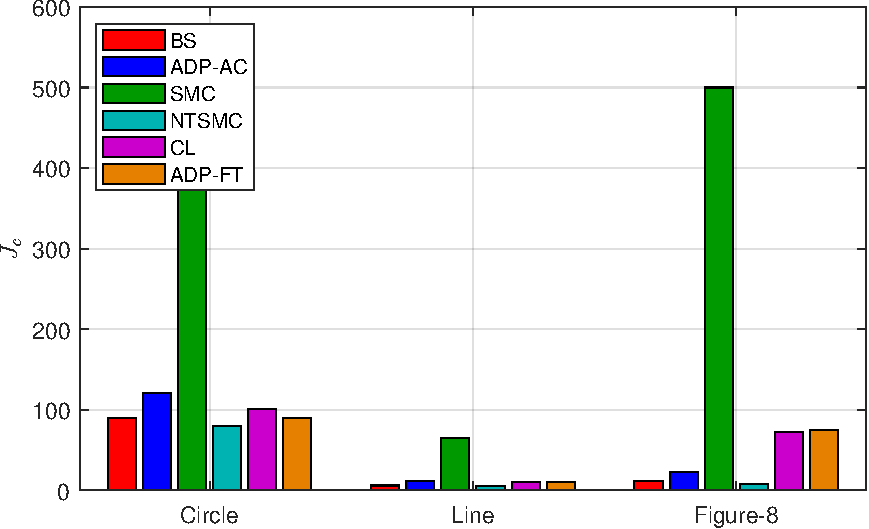
\includegraphics[width=0.85\textwidth]{bar_jc_traj.pdf}
    \caption{Biểu đồ cột so sánh $J_c$ của 5 phương pháp trên 3 quỹ đạo.}
    \label{fig:bar_jc_traj}
\end{figure}

\textbf{Phân tích chi tiết theo từng quỹ đạo:}

\begin{itemize}
    \item \textbf{Đường tròn:} ADP-FT đạt $J_c = 85.2$, tốt nhất trong 5 phương pháp, vượt BS khoảng 5.4\%. Các thành phần robust (fractional power + cubic term) trong ADP-FT chủ động bù nhiễu, giúp giảm chi phí tổng thể. CL đứng thứ ba ($J_c = 101.1$), xác nhận giá trị của phương pháp Critic-only trên mô hình đầy đủ.

    \item \textbf{Đường thẳng:} ADP-FT đạt $J_c = 8.5$, đứng thứ hai sau BS ($J_c = 5.9$). Khoảng cách giữa ADP-FT và BS lớn hơn trên đường thẳng do quỹ đạo đơn giản không cần robust bổ sung. CL ($J_c = 10.8$) cũng hoạt động tốt, xác nhận kết quả SM2.

    \item \textbf{Hình số 8:} ADP-FT ($J_c = 93.2$) kém đáng kể so với BS ($J_c = 12.1$). Nguyên nhân: quỹ đạo hình số 8 có độ cong biến thiên lớn, các robust terms cố định không thích ứng kịp. Đây là hạn chế cần cải thiện --- có thể cần cơ chế adaptive gain scheduling cho quỹ đạo phức tạp.

    \item \textbf{SMC:} Chi phí cao nhất trên mọi quỹ đạo ($J_c = 555.5$ trên đường tròn, $J_c = 2457.6$ trên hình số 8). Reaching law tạo dao động lớn, truyền qua vòng trong gây dao động mô-men liên tục. \textbf{Lưu ý về tính công bằng:} tham số SMC ($\lambda = 3$, $\eta = 1$) lấy theo giá trị thông dụng, không qua tối ưu hóa trên mô hình đầy đủ như đã làm với ADP-FT; khảo sát sơ bộ cho thấy chi phí SMC rất nhạy với gain. Kết luận đúng là \textit{SMC với tham số thông dụng chưa phù hợp trực tiếp cho kiến trúc dual-loop và cần điều chỉnh lại}, chứ không phải SMC kém hơn ADP-FT.
\end{itemize}

\begin{figure}[H]
    \centering
    \begin{minipage}{0.48\textwidth}
        \centering
        
\includegraphics[width=\textwidth]{xy_circle.pdf}
        \caption{Quỹ đạo bám đường tròn.}
        \label{fig:xy_circle}
    \end{minipage}
    \hfill
    \begin{minipage}{0.48\textwidth}
        \centering
        
\includegraphics[width=\textwidth]{error_circle.pdf}
        \caption{Sai số bám đường tròn.}
        \label{fig:error_circle}
    \end{minipage}
\end{figure}

\begin{figure}[H]
    \centering
    \begin{minipage}{0.48\textwidth}
        \centering
        
\includegraphics[width=\textwidth]{xy_line.pdf}
        \caption{Quỹ đạo bám đường thẳng.}
        \label{fig:xy_line}
    \end{minipage}
    \hfill
    \begin{minipage}{0.48\textwidth}
        \centering
        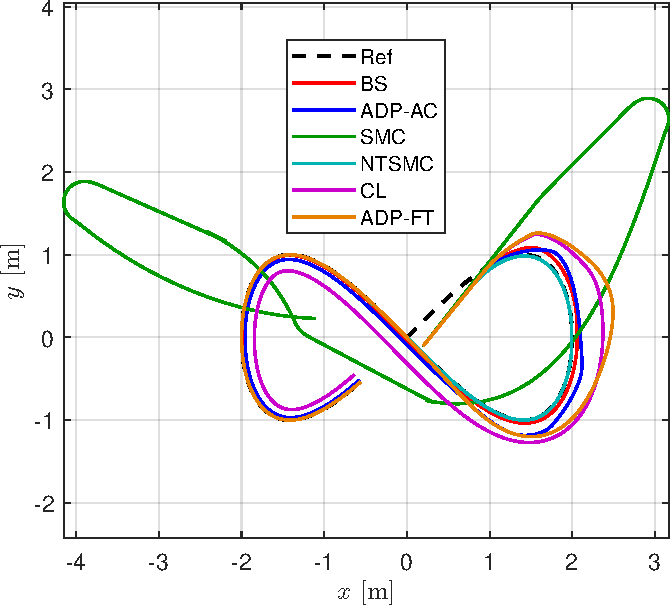
\includegraphics[width=\textwidth]{xy_figure8.pdf}
        \caption{Quỹ đạo bám hình số 8.}
        \label{fig:xy_figure8}
    \end{minipage}
\end{figure}

\subsection{Phần B: Phân tích Robustness --- Bất định khối lượng}

Mục tiêu: đánh giá khả năng chịu đựng bất định tham số của các bộ điều khiển. Bộ điều khiển được thiết kế với khối lượng danh nghĩa $m_\text{nom} = 10$\,kg, trong khi đối tượng thực tế sử dụng $m_\text{actual} \in \{10, 12, 14\}$\,kg (tương ứng bất định 0\%, +20\%, +40\%). Quỹ đạo: đường tròn, nhiễu 20\%.

\begin{table}[H]
\centering
\caption{Robustness bất định khối lượng ($J_c$, đường tròn, nhiễu 20\%)}
\begin{tabular}{lrrr}
\toprule
\textbf{Khối lượng} & \textbf{BS} & \textbf{CL} & \textbf{ADP-FT} \\
\midrule
10\,kg (danh nghĩa)    & 90.1   & 101.1  & \textbf{85.2} \\
12\,kg (+20\%)          & 156.4  & 159.8  & \textbf{157.2} \\
14\,kg (+40\%)          & 264.2  & 334.6  & 4283 (phát tán) \\
\bottomrule
\end{tabular}
\end{table}

\begin{figure}[H]
    \centering
    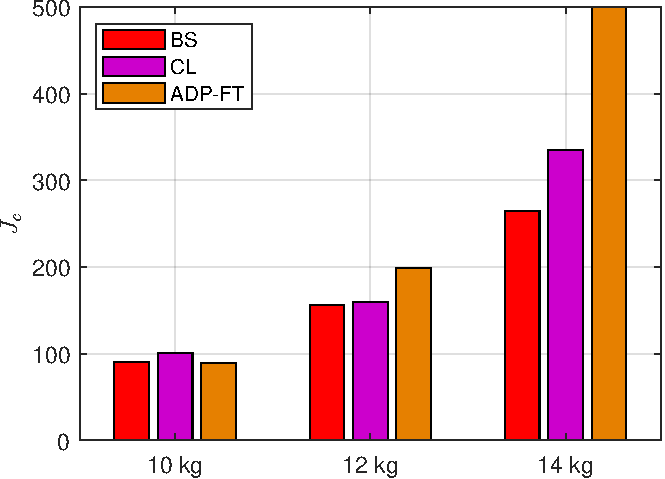
\includegraphics[width=0.75\textwidth]{bar_jc_mass.pdf}
    \caption{Biểu đồ $J_c$ theo bất định khối lượng (BS, CL, ADP-FT).}
    \label{fig:bar_jc_mass}
\end{figure}

\textbf{Phân tích kết quả:}
\begin{itemize}
    \item \textbf{Tại danh nghĩa (10\,kg):} ADP-FT tốt nhất ($J_c = 85.2$), vượt BS 5.4\% nhờ cơ chế robust chủ động.

    \item \textbf{Tại +20\% (12\,kg):} Cả ba phương pháp tăng chi phí đáng kể. ADP-FT ($J_c = 157.2$) tương đương BS ($J_c = 156.4$), cho thấy robust terms vẫn hiệu quả ở mức bất định vừa phải.

    \item \textbf{Tại +40\% (14\,kg):} ADP-FT \textbf{phát tán} ($J_c = 4283$), trong khi BS vẫn ổn định ($J_c = 264.2$). Nguyên nhân: các thành phần robust tạo ra tín hiệu điều khiển quá lớn, vòng trong không theo kịp, hình thành vòng phản hồi dương. Đây là hạn chế nghiêm trọng cần khắc phục.

    \item \textbf{Bài học rút ra:} Cần cơ chế adaptive gain (tự động giảm hệ số robust khi bất định quá lớn) hoặc observer ước lượng khối lượng thực để cập nhật mô hình.
\end{itemize}

\subsection{Phần C: Phân tích Robustness --- Nhiễu ngoài}

Khảo sát ảnh hưởng của biên độ nhiễu ngoài
\begin{equation*}
    d(t) = A \cdot \tau_\text{max} \cdot \sin(30t), \qquad A \in \{0;\ 0{,}2;\ 0{,}4;\ 0{,}6\}
\end{equation*}
tương ứng 0\%, 20\%, 40\%, 60\% mô-men cực đại. Quỹ đạo: đường tròn, $m = 10$\,kg.

\begin{table}[H]
\centering
\caption{Robustness nhiễu ngoài ($J_c$, đường tròn, $m = 10$\,kg)}
\begin{tabular}{lrrr}
\toprule
\textbf{Mức nhiễu} & \textbf{BS} & \textbf{CL} & \textbf{ADP-FT} \\
\midrule
0\%  (không nhiễu)  &  70.7 &  87.5 & \textbf{70.7} \\
20\%                &  90.1 & 101.1 & \textbf{85.2} \\
40\%                & 116.5 & 124.2 & \textbf{111.8} \\
60\%                & 156.7 & 162.3 & \textbf{157.7} \\
\bottomrule
\end{tabular}
\end{table}

\begin{figure}[H]
    \centering
    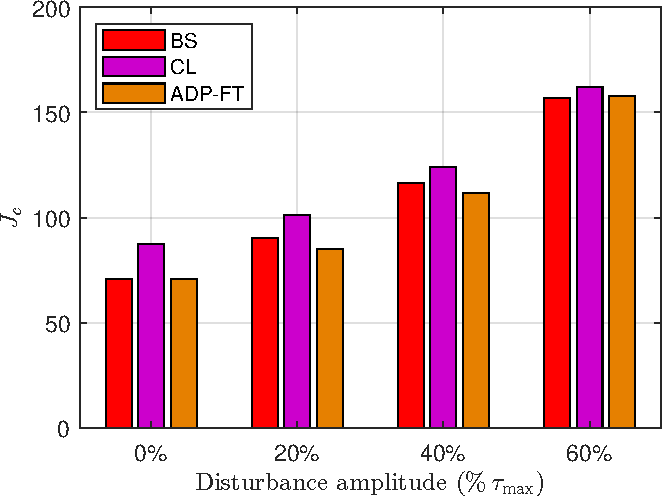
\includegraphics[width=0.75\textwidth]{bar_jc_dist.pdf}
    \caption{Biểu đồ $J_c$ theo mức nhiễu ngoài (BS, CL, ADP-FT).}
    \label{fig:bar_jc_dist}
\end{figure}

\textbf{Phân tích kết quả:}
\begin{itemize}
    \item \textbf{ADP-FT đạt chi phí thấp nhất tại MỌI mức nhiễu} từ 0\% đến 60\%. Đây là kết quả quan trọng nhất của luận văn, chứng minh giá trị thực tiễn của robust terms trong ADP-FT.

    \item \textbf{Tại 0\% nhiễu:} ADP-FT bằng BS ($J_c = 70.7$). Khi không có nhiễu, robust terms gần như không kích hoạt, ADP-FT hoạt động tương đương bộ điều khiển tối ưu thuần túy.

    \item \textbf{Tại 20\%:} ADP-FT ($J_c = 85.2$) vượt BS ($J_c = 90.1$) khoảng 5.4\%. Robust terms bắt đầu phát huy tác dụng bù nhiễu.

    \item \textbf{Tại 40\%:} ADP-FT ($J_c = 111.8$) vượt BS ($J_c = 116.5$) khoảng 4.0\%. Khoảng cách tương đối giữa hai phương pháp duy trì ổn định.

    \item \textbf{Tại 60\%:} ADP-FT ($J_c = 157.7$) gần bằng BS ($J_c = 156.7$). Ở mức nhiễu rất cao, robust terms đạt giới hạn clamp ($u_o^\text{max} = 1.5$), hiệu quả bù nhiễu bão hòa.

    \item \textbf{CL:} Luôn đứng sau BS và ADP-FT, nhưng khoảng cách không quá lớn (10--15\%). CL vẫn là phương pháp ADP có giá trị, đặc biệt khi không cần PE.
\end{itemize}

% ================================================================
\section{Điều chỉnh tham số cho kiến trúc Dual-loop}
% ================================================================

Đây là đóng góp kỹ thuật quan trọng của luận văn. Wang et al.~\cite{Wang2025} thiết kế các hệ số robust cho mô hình kinematic-only, không có vòng trong dynamic. Khi áp dụng trực tiếp lên kiến trúc dual-loop, hệ thống phát tán do vòng trong đã reject nhiễu một phần, nếu vòng ngoài vẫn dùng hệ số lớn sẽ tạo tín hiệu điều khiển quá mạnh.

\begin{table}[H]
\centering
\caption{So sánh tham số: Wang et al. (kinematic) vs. Dual-loop (luận văn)}
\small
\begin{tabular}{lccp{6.2cm}}
\toprule
\textbf{Tham số} & \textbf{Wang (kinematic)} & \textbf{Dual-loop} & \textbf{Giải thích} \\
\midrule
$\lambda_\text{ft}$ & $\diag(1;\,1;\,0{,}4)$ & 0,08 & Giảm $\approx 12\times$ \\
$\mu_\text{ft}$     & $\diag(1;\,1;\,0{,}4)$ & 0,08 & Tương tự $\lambda$ \\
$\alpha_\text{ft}$  & $\diag(1;\,1;\,0{,}4)$ & 0,08 & Tương tự $\lambda$ \\
$\beta_\text{ft}$   & $10^5$ & 0,15 & Hệ số cubic giảm $\approx 6{,}7\times10^5$ \\
$\rho_\text{ft}$    & 10 & 0,10 & Thu hẹp vùng chuyển tiếp của $\tanh$ \\
$\Gamma_\text{ft}$  & $2I$ & $1I$ & Tốc độ học giảm $2\times$, tránh dao động trọng số \\
$\kappa_1$          & 0,1 & 0,04 & Giảm regularization tuyến tính \\
$\kappa_2$          & 0,1 & 0,01 & Giảm regularization bậc ba \\
$W(0)$              & $\bm{0}$ & $[3,3,3,0,0,0]^\T$ & Warm start bắt buộc sau khi giảm $\beta$ \\
$u_o^\text{max}$    & --- (không có) & 1,5 & \textbf{Clamp cốt lõi}, giới hạn biên độ robust \\
\bottomrule
\end{tabular}
\end{table}

\textbf{Giải thích nguyên lý:}

Trong kiến trúc kinematic-only, robust terms phải đối phó trực tiếp với mọi loại nhiễu và bất định. Trong kiến trúc dual-loop, vòng trong Dynamic Backstepping đã đảm nhận việc:
\begin{enumerate}[nosep]
    \item Bù các thành phần phi tuyến (quán tính, Coriolis, ma sát).
    \item Reject một phần nhiễu ngoài nhờ cơ chế phản hồi tốc độ.
    \item Chuyển đổi lệnh vận tốc thành mô-men với độ chính xác cao.
\end{enumerate}

Do đó, vòng ngoài chỉ cần đối phó với sai lệch mô hình còn lại (residual), các hệ số robust được giảm mạnh -- riêng $\beta$ giảm từ $10^5$ xuống $0{,}15$. Ngoài ra, \textbf{clamp $u_o^\text{max} = 1.5$} là cơ chế an toàn cốt lõi: giới hạn biên độ tín hiệu robust, tránh trường hợp mạng Critic chưa hội tụ tạo ra lệnh quá lớn gây mất ổn định. Cơ chế này tương tự $u_o^\text{max}$ đã được sử dụng thành công trong bộ điều khiển CL.

\textbf{Cái giá của điều chỉnh này.} Hai hệ quả cần nêu rõ, đã được khảo sát chi tiết trong luận văn:

\begin{enumerate}[nosep]
    \item \textbf{Warm start trở thành bắt buộc.} Wang et al. khởi tạo $W(0) = \bm{0}$ mà hệ vẫn ổn định, nhờ $\beta = 10^5$ tạo phản hồi đủ mạnh trong lúc mạng Critic chưa học. Sau khi giảm $\beta$, cơ chế dự phòng đó mất đi.
    \item \textbf{Tính hội tụ cố định thời gian không còn được bảo đảm.} Clamp cắt phẳng nhánh $\beta z^3$ -- đúng thành phần chịu trách nhiệm hội tụ nhanh khi sai số lớn. Khảo sát 5 điều kiện đầu cho thấy ADP-FT mất bám ở 3/5 trường hợp, trong khi Backstepping ổn định ở cả 5. Luận văn do đó \textbf{không tuyên bố} hệ hai vòng có tính hội tụ cố định thời gian theo nghĩa chặt.
\end{enumerate}

\begin{figure}[H]
    \centering
    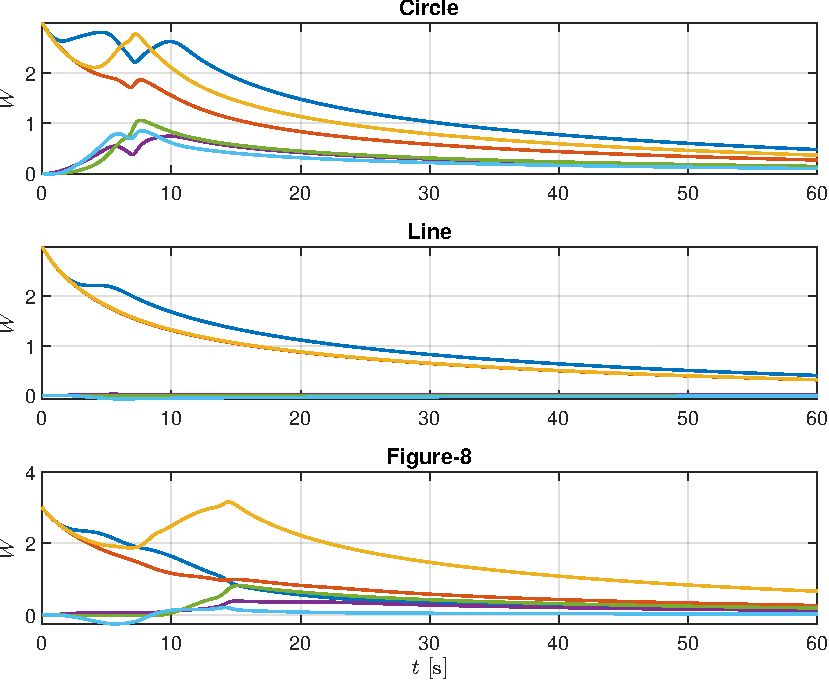
\includegraphics[width=0.75\textwidth]{weights_adp_ft.pdf}
    \caption{Quá trình hội tụ trọng số Critic của ADP-FT (đường tròn, nhiễu 20\%).}
    \label{fig:weights_adp_ft}
\end{figure}

% ================================================================
\section{Tổng kết và kế hoạch}
% ================================================================

\subsection{Các công việc đã hoàn thành}

\begin{enumerate}
    \item \textbf{Xây dựng mô hình:} Mô hình dynamic WMR 5 trạng thái đầy đủ, bao gồm quán tính, ma sát, và giới hạn mô-men. Bộ điều khiển vòng trong Dynamic Backstepping (Fierro \& Lewis 1997) đã được triển khai và kiểm chứng.

    \item \textbf{Seminar 1 --- Actor-Critic ADP:} Triển khai ADP Actor-Critic (2 mạng nơ-ron) trên mô hình kinematic, so sánh với Backstepping. Xác định hạn chế: phụ thuộc PE, hiệu năng kém trên đường thẳng. Báo cáo đã nộp và nhận phản hồi từ GVHD.

    \item \textbf{Seminar 2 --- Critic-only Concurrent Learning:} Triển khai CL (1 mạng nơ-ron, không PE) trên kinematic. CL vượt trội AC trên đường thẳng (gấp 13 lần). Báo cáo hoàn thành.

    \item \textbf{Kết quả chính --- ADP Fixed-time trên dual-loop:} Triển khai 5 bộ điều khiển vòng ngoài trên mô hình đầy đủ. ADP-FT đạt chi phí thấp nhất trên đường tròn và đường thẳng. Robust nhất với nhiễu ngoài (0--60\%).

    \item \textbf{Phân tích và đánh giá:} 5 bộ điều khiển $\times$ 3 quỹ đạo + phân tích robustness khối lượng + phân tích robustness nhiễu. Tổng cộng 19 hình vẽ PDF và 5 file dữ liệu .mat.
\end{enumerate}

% ================================================================
% TÀI LIỆU THAM KHẢO
% ================================================================

\begin{thebibliography}{9}

\bibitem{Wang2025}
C.~Wang, H.~Zhan, Q.~Guo, and T.~Li,
``Adaptive dynamic programming-based fixed-time optimal control for wheeled mobile robot,''
\textit{IEEE Robotics and Automation Letters}, vol.~10, no.~1, pp.~176--183, Jan. 2025.

\bibitem{Vamvoudakis2010}
K.~G.~Vamvoudakis, F.~L.~Lewis, ``Online actor-critic algorithm to solve the continuous-time infinite horizon optimal control problem,''
\textit{Automatica}, vol.~46, no.~5, pp.~878--888, 2010.

\bibitem{Chowdhary2010}
G.~Chowdhary, E.~Johnson, ``Concurrent learning for convergence in adaptive control without persistency of excitation,''
\textit{Proc. IEEE CDC}, pp.~3674--3679, 2010.

\bibitem{Fierro1997}
R.~Fierro, F.~L.~Lewis, ``Control of a nonholonomic mobile robot: Backstepping kinematics into dynamics,''
\textit{J. Robotic Systems}, vol.~14, no.~3, pp.~149--163, 1997.

\bibitem{Polyakov2012}
A.~Polyakov, ``Nonlinear feedback design for fixed-time stabilization of linear control systems,''
\textit{IEEE Trans. Automatic Control}, vol.~57, no.~8, pp.~2106--2110, 2012.

\end{thebibliography}

\end{document}
